%----------------------------------------------------------------------------------------
%	PACKAGES AND OTHER DOCUMENT CONFIGURATIONS
%----------------------------------------------------------------------------------------

\documentclass[11pt]{scrartcl} % Font size

%%%%%%%%%%%%%%%%%%%%%%%%%%%%%%%%%%%%%%%%%
% Wenneker Assignment
% Structure Specification File
% Version 2.0 (12/1/2019)
%
% This template originates from:
% http://www.LaTeXTemplates.com
%
% Authors:
% Vel (vel@LaTeXTemplates.com)
% Frits Wenneker
%
% License:
% CC BY-NC-SA 3.0 (http://creativecommons.org/licenses/by-nc-sa/3.0/)
% 
%%%%%%%%%%%%%%%%%%%%%%%%%%%%%%%%%%%%%%%%%

%----------------------------------------------------------------------------------------
%	PACKAGES AND OTHER DOCUMENT CONFIGURATIONS
%----------------------------------------------------------------------------------------

\usepackage{amsmath, amsfonts, amsthm} % Math packages

\usepackage{listings} % Code listings, with syntax highlighting

\usepackage{graphicx} % Required for inserting images

\usepackage{booktabs} % Required for better horizontal rules in tables

\usepackage{dirtytalk} % Required for quoting.

\usepackage{float} % Added for hard placement of images.

\usepackage[dvipsnames]{xcolor} % Added for extra colors.

\usepackage{tikz} % For colored boxes and more.

\numberwithin{equation}{section} % Number equations within sections (i.e. 1.1, 1.2, 2.1, 2.2 instead of 1, 2, 3, 4)
\numberwithin{figure}{section} % Number figures within sections (i.e. 1.1, 1.2, 2.1, 2.2 instead of 1, 2, 3, 4)
\numberwithin{table}{section} % Number tables within sections (i.e. 1.1, 1.2, 2.1, 2.2 instead of 1, 2, 3, 4)

\usepackage{enumitem} % Required for list customisation
\setlist{noitemsep} % No spacing between list items

\usepackage[main=greek, english]{babel}

%----------------------------------------------------------------------------------------
%	DOCUMENT MARGINS
%----------------------------------------------------------------------------------------

\usepackage{geometry} % Required for adjusting page dimensions and margins

\geometry{
	paper=a4paper, % Paper size, change to letterpaper for US letter size
	top=2.5cm, % Top margin
	bottom=3cm, % Bottom margin
	left=3cm, % Left margin
	right=3cm, % Right margin
	headheight=0.75cm, % Header height
	footskip=1.5cm, % Space from the bottom margin to the baseline of the footer
	headsep=0.75cm, % Space from the top margin to the baseline of the header
	%showframe, % Uncomment to show how the type block is set on the page
}

%----------------------------------------------------------------------------------------
%	FONTS
%----------------------------------------------------------------------------------------

\usepackage[utf8]{inputenc} % Required for inputting international characters
\usepackage[T1]{fontenc} % Output font encoding for international characters

\usepackage{XCharter} % Use the XCharter fonts


%----------------------------------------------------------------------------------------
%	SECTION TITLES
%----------------------------------------------------------------------------------------

\usepackage{sectsty} % Allows customising section commands

\sectionfont{\vspace{6pt}\centering\normalfont\scshape} % \section{} styling
\subsectionfont{\normalfont\bfseries} % \subsection{} styling
\subsubsectionfont{\normalfont\itshape} % \subsubsection{} styling
\paragraphfont{\normalfont\scshape} % \paragraph{} styling

%----------------------------------------------------------------------------------------
%	HEADERS AND FOOTERS
%----------------------------------------------------------------------------------------

\usepackage{scrlayer-scrpage} % Required for customising headers and footers

\ohead*{} % Right header
\ihead*{} % Left header
\chead*{} % Centre header

\ofoot*{} % Right footer
\ifoot*{} % Left footer
\cfoot*{\pagemark} % Centre footer

\newcommand{\img}[1] % maybe add a caption to this
{
    \begin{center}
        \fcolorbox{black}{white}{\includegraphics[width=\textwidth]{#1}}
    \end{center}

}

% Helper Macros

\newcommand{\en}[1]{\foreignlanguage{english}{#1}}
\newcommand{\src}[1]{{\texttt{#1}}}


% Extra Formatting

\setlength{\parindent}{0em}
\setlength{\parskip}{0em}


% Code Listing Style

\lstdefinestyle{code}{
  belowcaptionskip=1\baselineskip,
  breaklines=true,
  frame=LRTB,
  xleftmargin=\parindent,
  showstringspaces=false,
  basicstyle=\ttfamily,
  keywordstyle=\bfseries\color{green!40!black},
  commentstyle=\itshape\color{purple!40!black},
  identifierstyle=\color{black},
  stringstyle=\color{orange},
}


\newcommand{\lstcode}[3]
{
    \begin{otherlanguage}{english}
    \lstinputlisting[language=#2, frame=single, style=code, caption=#3]{#1}
    \end{otherlanguage}
}
 % Include the file specifying the document structure and custom commands
\usepackage{multirow}
\usepackage{array}
\usepackage{subcaption}
\usepackage{textcomp}
\usepackage{algorithm}
\usepackage{algpseudocode}

\usetikzlibrary{positioning}

% Define a macro to create a table with fixed column widths
\newcolumntype{C}[1]{>{\centering\arraybackslash}p{#1}}

\usepackage{hyperref}
\hypersetup{
    colorlinks=true,
    linkcolor=blue,
    filecolor=magenta,      
    urlcolor=cyan,
}

\definecolor{diffstart}{named}{Apricot}
\definecolor{diffincl}{named}{Green}
\definecolor{diffrem}{named}{Red}

\usepackage{listings}
  \lstdefinelanguage{diff}{
    basicstyle=\ttfamily\small,
    morecomment=[f][\color{diffstart}]{@@},
    morecomment=[f][\color{diffincl}]{+\ },
    morecomment=[f][\color{diffrem}]{-\ },
  }

\definecolor{codegreen}{rgb}{0,0.6,0}
\definecolor{codegray}{rgb}{0.5,0.5,0.5}
\definecolor{codepurple}{rgb}{0.58,0,0.82}
\definecolor{backcolour}{rgb}{0.95,0.95,0.92}
\definecolor{codeblue}{rgb}{0,0,0.8}

\lstdefinestyle{mystyle}{
    backgroundcolor=\color{backcolour},   
    commentstyle=\color{codegreen},
    keywordstyle=\color{codeblue},
    numberstyle=\tiny\color{codegray},
    stringstyle=\color{codepurple},
    basicstyle=\ttfamily\footnotesize,
    breakatwhitespace=false,         
    breaklines=true,                 
    captionpos=b,                    
    keepspaces=true,                 
    numbers=left,                    
    numbersep=5pt,                  
    showspaces=false,                
    showstringspaces=false,
    showtabs=false,                  
    tabsize=2
}
\usepackage{tocloft}
\renewcommand{\cftsecfont}{\normalfont}
\renewcommand{\cftsecpagefont}{\normalfont}
\addto\captionsgreek{\renewcommand{\contentsname}{\normalfont Περιεχόμενα}}

\lstset{style=mystyle}

%----------------------------------------------------------------------------------------
%	TITLE SECTION
%----------------------------------------------------------------------------------------

\title{	
	\normalfont\normalsize
	\textsc{Πανεπιστήμιο Πατρών, Τμήμα Μηχανικών ΗΥ και Πληροφορικής \\Τεχνολογία λογισμικού 2023}\\ % Your university, school and/or department name(s)
	\vspace{25pt} % Whitespace
	\rule{\linewidth}{0.5pt}\\ % Thin top horizontal rule
	\vspace{20pt} % Whitespace
    {\Large Team Plan v0.1}\\ % The assignment title
	\vspace{12pt} % Whitespace
	\rule{\linewidth}{0.5pt}\\ % Thick bottom horizontal rule
	\vspace{12pt} % Whitespace
    
\includegraphics[width=0.7\textwidth]{../../brand/png/logo-transparent.png}
        \rule{\linewidth}{2pt}
}
\author{
Βασίλειος Τσούλος \thanks{Editor} \\UP1072605 \and Κωνσταντίνος Γιακαλλής \thanks{Co-editor} \\UP1072533
\and \hspace{-1ex} Ιωάννης Παναρίτης \\ \hspace{-1ex} UP1072632  \and Νικόλαος Χαλκιόπουλος \\UP1072572
}



\date{} % Today's date (\today) or a custom date

%----------------------------------------------------------------------------------------
%	DOCUMENT
%----------------------------------------------------------------------------------------

\bibliographystyle{ieeetr}
\addto\captionsgreek{\renewcommand{\refname}{Αναφορές}}


\begin{document}

\maketitle
\pagebreak

\tableofcontents
\Large

\section{Εργαλεία που θα χρησιμοποιήσουμε}
\begin{itemize}
    \item Συγγραφή Κειμένου: Overleaf
    \item Γραφιστικά και mock ups: Gimp
    \item Γλώσσα προγραματισμού: Python
    \item Ide: Visual Studio Code
    \item Δημιουργία Gantt: Teamgantt
    \item Δημιουργία Pert: Visual paradigm
    \item Επικοινωνία Μελών: Discord
    \item Διαμοιρασμός και παρακολούθηση διαδικασίας ανάπτυξης: Github
\end{itemize}
\pagebreak

\section{Χρονοπρογραμματισμός έργου}
\begin{table}[ht]
\centering
\resizebox{\textwidth}{!}
{
\Large
\begin{tabular}{|c | p{0.5\linewidth} | c | c | c | c |}
\hline
Τυπικό υποέργο & Περιγραφή                                                                                                         & Εξαρτήσεις & Αισιόδοξη (μέρες) & Κανονική (μέρες) & Απαισιόδοξη (μέρες) \\ \hline
ΤΥ1            & Αρχικο brainstorming και υλοποίηση   project description                                                          & -          & 3         & 4        & 7           \\ \hline
TΥ2            & Περαιτέρω   ανάπτυξη ιδέας και δομή έργου και υλοποίηση project plan                                              & ΤΥ1        & 2         & 3        & 4           \\ \hline
TΥ3            & Ανάλυση ρίσκων   για την υλοποίηση του έργου, υλοποίηση risk assesment                                            & ΤΥ2        & 1         & 1        & 2           \\ \hline
TΥ4            & Καταμερισμός εργασιών,πόρων   και mapping της εργασιας του project, team plan                                     & ΤΥ2        & 1         & 2        & 3           \\ \hline
TΥ5            & Καταγραφή features και ανάλυση χρηστών εφαρμογής για την   κατασκευη και ανάθεση use cases                        & ΤΥ2        & 7         & 8        & 9           \\ \hline
TΥ6            & Κατηγοριοποίηση   του έργου και εκπόνηση κλάσεων για τη δημιουργία του domain model                               & TΥ2        & 3         & 4        & 5           \\ \hline
TΥ7            & Δημιουργία robustness diagrams των use cases για περεταιρω   αναλυση τους                                         & TΥ5        & 10        & 15       & 20          \\ \hline
TΥ8            & Αναθεωρηση use   cases με βάση τα robustness diagrams                                                             & TΥ3, TY6   & 6         & 7        & 8           \\ \hline
TΥ9            & Αναθεώρηση domain model με βάση τα   robustness diagrams                                                          & ΤΥ4, TY6   & 6         & 7        & 8           \\ \hline
TΥ10           & Αρχή συγγραφής κώδικα έργουmilestone-done with implemetation and starting alpha                                   & ΤΥ9, TY10  & 10        & 20       & 25          \\ \hline
TΥ11           & Βασιζόμενοι στα use cases και   robustness diagrams υλοποιούμε τα sequence diagrams                               & ΤΥ10       & 10        & 15       & 20          \\ \hline
TΥ12           & Αναθεώρηση domain models και πιθανώς   use cases με βαση sequence diagrams                                        & ΤΥ11       & 6         & 7        & 8           \\ \hline
TY13           & Βασισμένοι στο domain model και τον κώδικά μας αναπτύσσουμε το class diagram                                      & TY10       & 10        & 15       & 20          \\ \hline
TY14           & Δοκιμάζουμε και   τελειοποιούμε μια alpha version του κωδικά μας για υποβολή                                      & TY10,TY12  & 15        & 20       & 25          \\ \hline
TY15           & Αναθεώρηση και   βελτίωση όλων των εργαλείων και μοντέλων για την ανάπτυξη του έργου, παράδοση   τελικών αναφορών & TY13, TY14 & 25        & 30       & 35          \\ \hline
TY16           & Τελειοποίηση   της εφαρμογής και παρουσίαση της alpha version                                                     & TY13, TY14 & 25        & 30       & 35          \\ \hline       
\end{tabular}}
\end{table}
\pagebreak

\section{Gantt Chart}

Παρακάτω παρατίθεται ο χρονοπρογραμματισμός του έργου. Ως έναρξη του project έχει οριστεί η 1η Μαρτίου και ως λήξη η 6η Ιούλη.\\
% \vspace{1cm}
\begin{figure}[ht]
    \hspace{-3.3cm}
    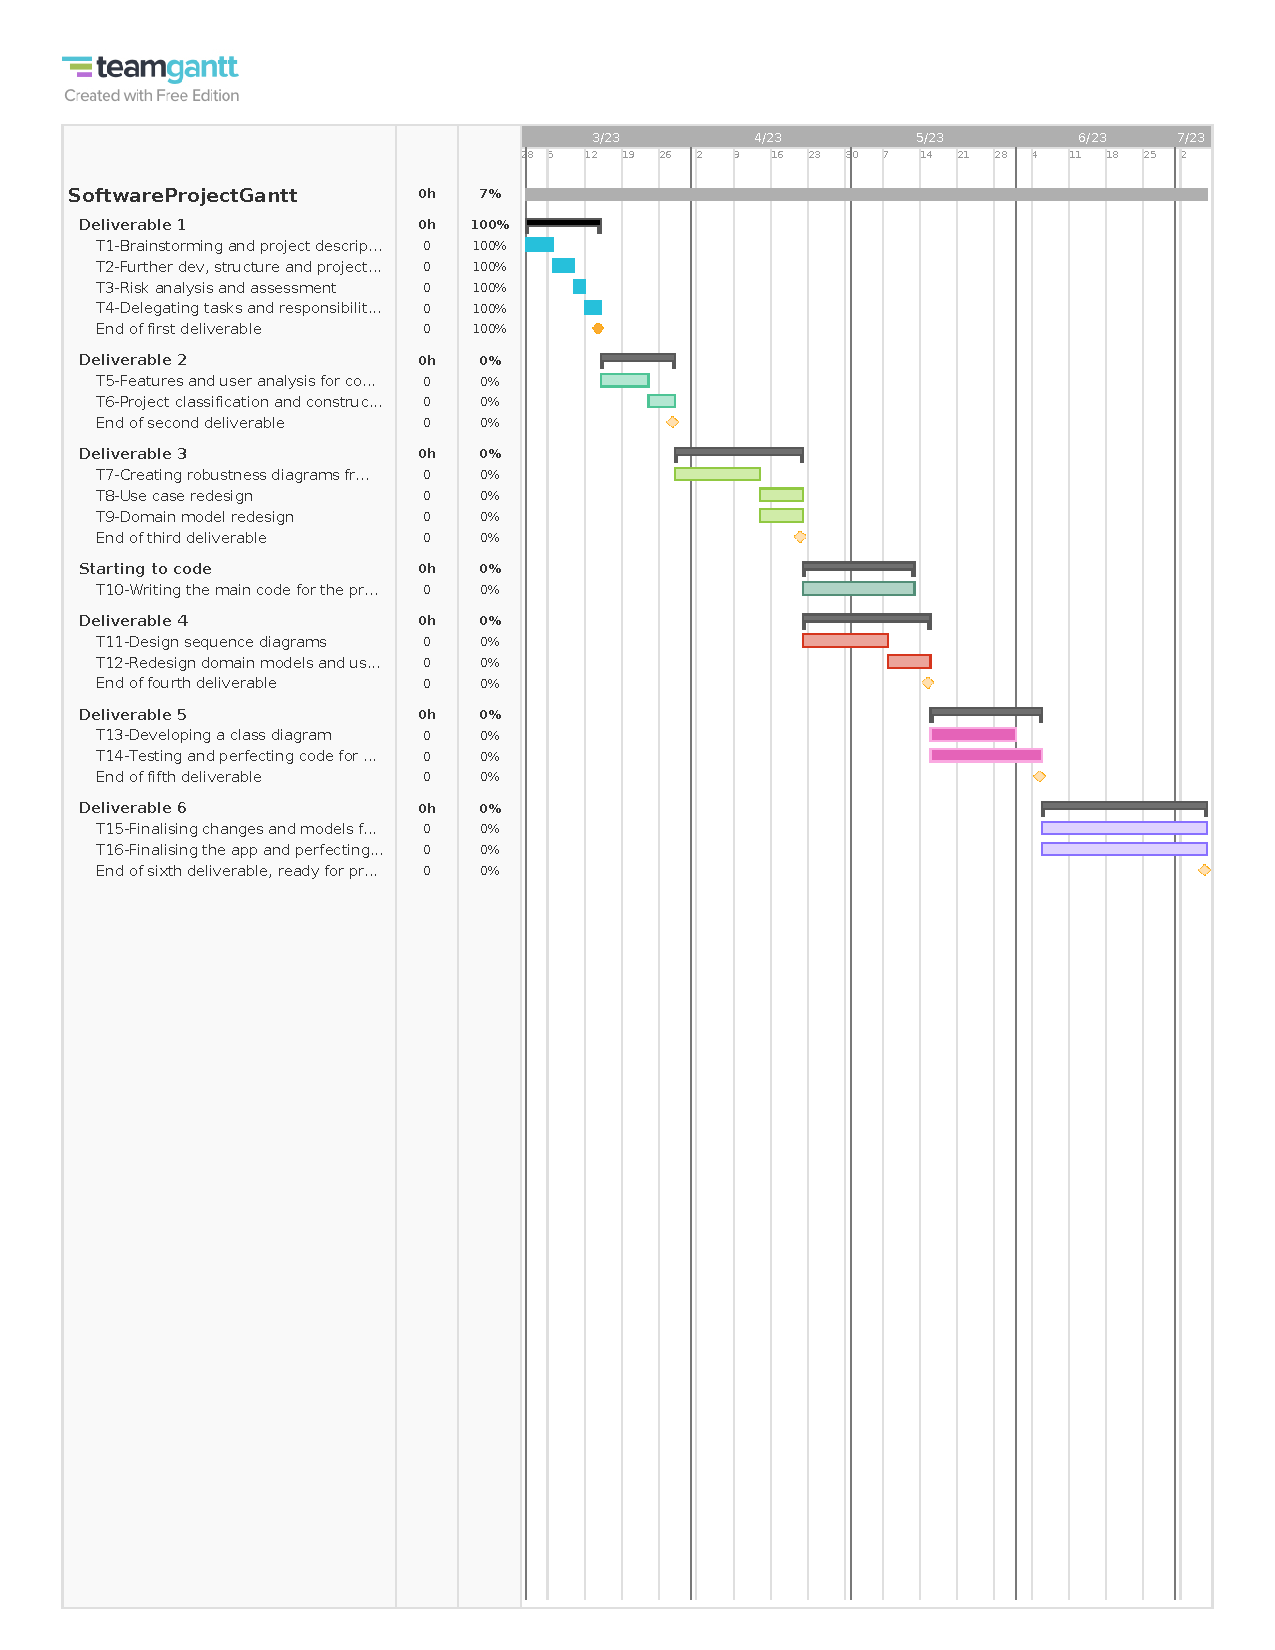
\includegraphics[trim = 0cm 12cm 0cm 2cm, clip]{docs/Team-plan/assets/GanttForProject.pdf}
    \caption{Gantt chart}
\end{figure}

Ως τυπικά υποέργα (tasks), είχαμε τα Τεχνικά Κείμενα που έπρεπε να παραδοθούν σε κάθε ένα από τα παραδοτέα. Τα tasks , φαίνονται στο Gantt διάγραμμα.
Στο τέλος κάθε παραδοτέου υπήρχε ένα Milestone. 

Συγκεκριμένα :
\begin{enumerate}
    \item Ανάλυση Απαιτήσεων Εφαρμογής (Requirements Engineering)
    \item Σχεδιασμός Γενικής Αρχιτεκτονικής και Λειτουργιών Συστήματος
    \item Επέκταση Αρχιτεκτονικής και Minimum Viable Product
    \item Testing Υλοποίησης
    \item Τελικές αλλαγές στο σύστημα και παράδοση στον πελάτη
\end{enumerate}

\section{Pert Chart}

\begin{figure}[ht]
    \hspace{-0.5cm}
    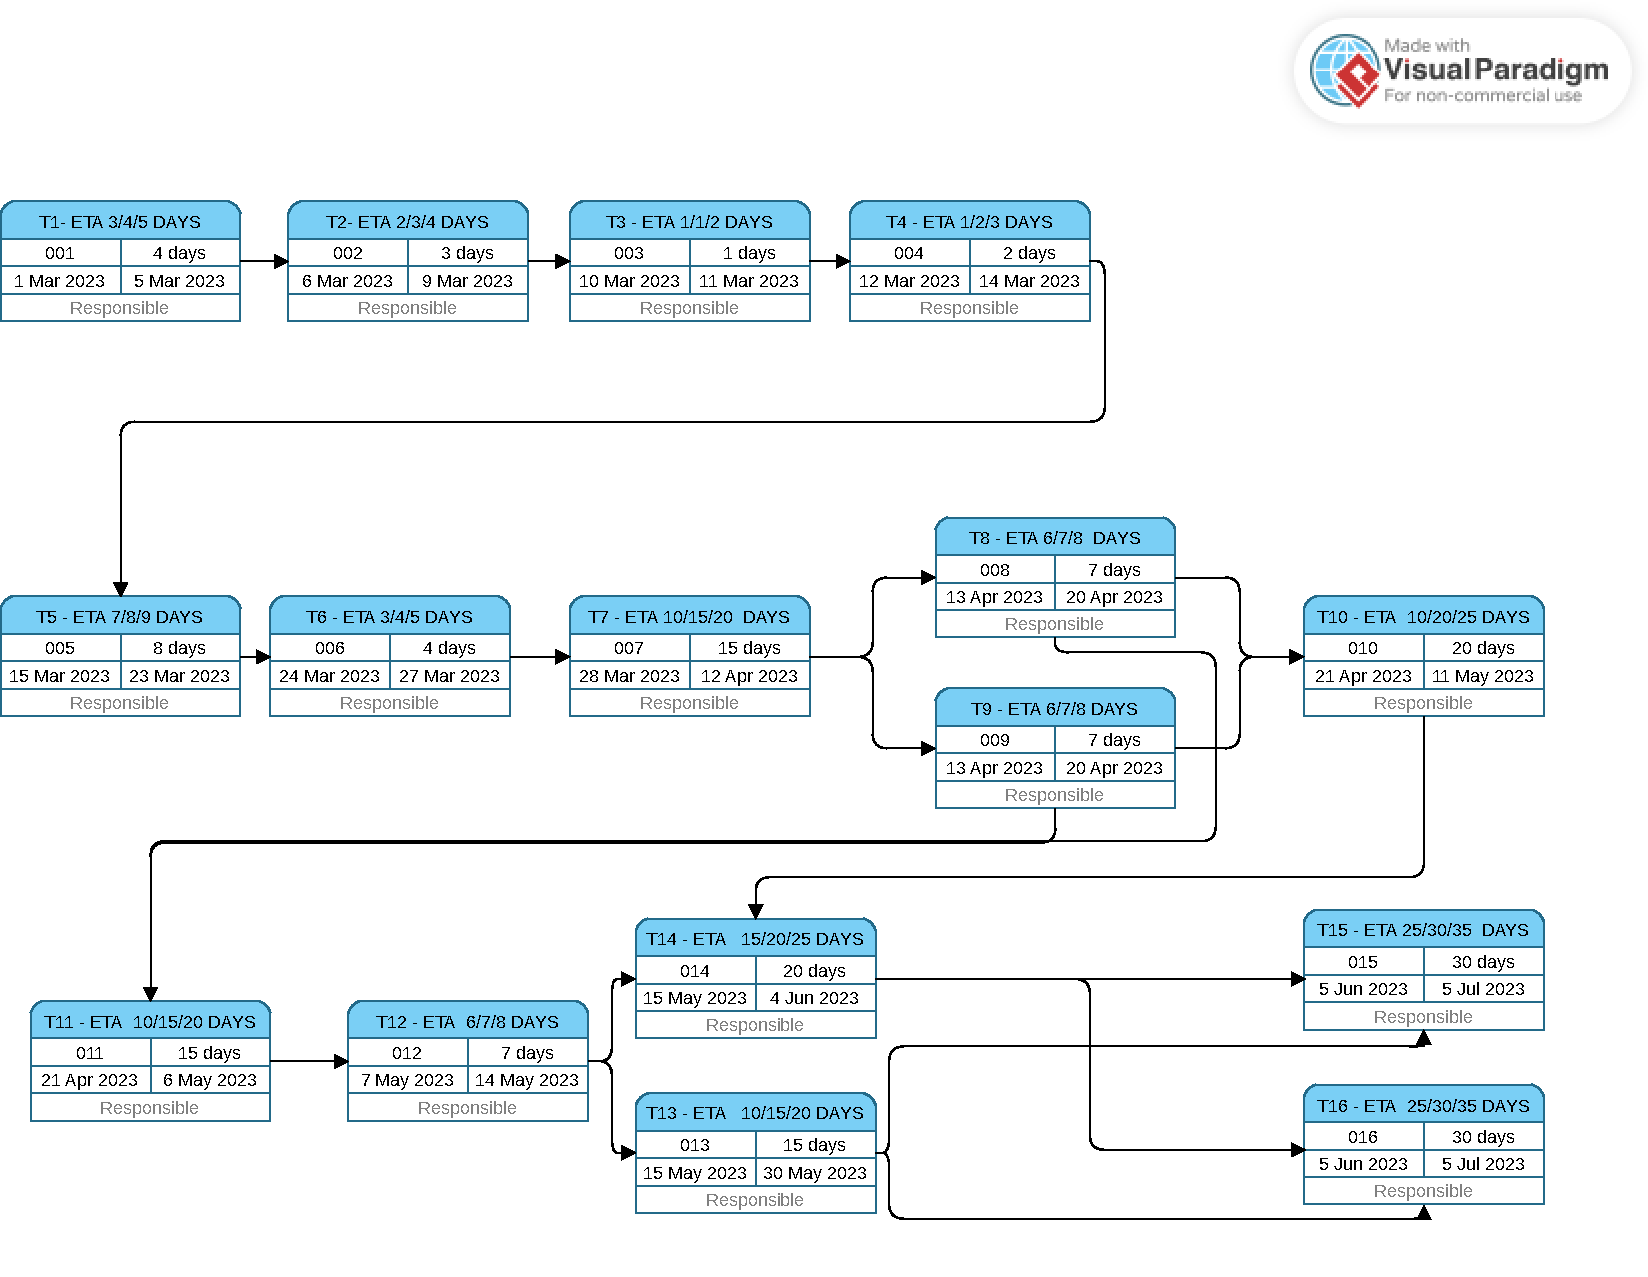
\includegraphics[width = 1.2\linewidth,trim = 0cm 0cm 0cm 2cm, clip]{docs/Team-plan/assets/pertForProject.pdf}
    \caption{Pert chart}
\end{figure}

\section{Στόχοι Ομάδας}
\begin{itemize}
    \item Ανάπτυξη ενός εύχρηστου και αποτελεσματικού εργαλείου που θα βοηθήσει τους ιδιοκτήτες οχημάτων να διατηρούν τα οχήματά τους σε καλή κατάσταση και να μειώνουν την ανάγκη για συχνές επισκευές.
    \item Να διασφαλιστεί ότι το εργαλείο είναι εύκολο στη χρήση και μπορεί να χρησιμοποιηθεί από οποιονδήποτε, ανεξάρτητα από το επίπεδο τεχνικών γνώσεων τους.
    \item Να διενεργηθούν εκτενή τεστ και να διασφαλιστεί ότι το εργαλείο είναι αξιόπιστο και ακριβές.
\end{itemize}

\section{Μέθοδος Εργασίας}
Στην πρώτη μας συνάντηση ορίστηκε η μέθοδος εργασίας μας, καθώς και ο αριθμός των εβδομαδιαίων συναντήσεων που θα θέλαμε να τηρηθούν καθόλη την διάρκεια του ΄Εργου.\\
Ομόφωνα αποφασίστηκε οτι σε κάθε συνάντηση θα αφιερώνουμε 10 λεπτά να επανεξετάζουμε τι έχει γίνει το διάστημα που πέρασε από την προηγούμενη συνάντηση, στην συνέχεια θα δίνουμε feedback σε ότι έχει ήδη προετοιμαστεί, ώστε να προχωρήσουμε σε οριστικοποίηση ή διόρθωση και τέλος θα θέτουμε τους στόχους μας για την επόμενη φορά χωρίζοντας τον φόρτο εργασίας ανάμεσα στα μέλη της ομάδας. \\
Ο αριθμός των σταθερών εβδομαδιαίων συναντήσεων ορίστηκε για 2, με φυσικά οποιαδήποτε έξτρα προσθήκη κριθεί απαραίητη κατά την διάρκεια ώστε να μείνουμε εντός χρονοδιαγράμματος. \\
Ως μέσο επικοινωνίας και planning ορίστηκε η πλατφόρμα Discord .Παράλληλα τα αρχεία κώδικα που θα επεξεργαζόμαστε καθόλη την διάρκεια του ΄Εργου θα βρίσκονται στο GitHub της ομάδας μας (https://github.com/basilis0606/MainTena)



% \bibliography{bibliography}

\end{document}
